\section{Синтез регулятора с заданной степенью устойчивости}

\subsection{Анализ системы}

Рассмотрим систему
\begin{equation}
    \dot x=Ax+Bu,\quad A=\begin{bmatrix}
        3&5&4\\
        -2&-4&-5\\
        2&2&3
    \end{bmatrix},\quad B=\begin{bmatrix}
        2\\-1\\1
    \end{bmatrix}.
    \label{eq:sys1}
\end{equation}
Cобственные числа матрицы $A$
\begin{equation*}
    \sigma(A)=\{\ 2\pm i,\ -2\ \}.
\end{equation*}
Рассмотрим матрицы Хаутуса и их ранги
\begin{equation*}
    H_1 = \begin{bmatrix}
        (2+ i) I - A & B
    \end{bmatrix} =
    \begin{bmatrix}
        -1 + i & -5 & -4 & 2 \\ 
         2 &  6 + i &  5 & -1 \\ 
        -2 & -2 & -1 + i &  1
    \end{bmatrix},
    \quad\text{rank}(H_1) = 3,
\end{equation*}
\begin{equation*}
    H_2 = \begin{bmatrix}
        (2- i) I - A & B
    \end{bmatrix} =
    \begin{bmatrix}
        -1 - i & -5 & -4 & 2 \\ 
         2 &  6 - i &  5 & -1 \\ 
        -2 & -2 & -1 - i &  1
    \end{bmatrix},
    \quad\text{rank}(H_2) = 3,
\end{equation*}
\begin{equation*}
    H_3 = \begin{bmatrix}
        -2 I - A & B
    \end{bmatrix} =
    \begin{bmatrix}
        -5 & -5 & -4 &  2 \\ 
         2 &  2 &  5 & -1 \\ 
        -2 & -2 & -5 &  1
    \end{bmatrix},
    \quad\text{rank}(H_3) = 2.
\end{equation*}
Как видно, система не полностью управляема, но стабилизируема, так как единственное
неуправляемое собственное число $-2$ отрицательно.

Если мы будем использовать регулятор вида $u=-Kx$, то не получится получить
любую степень устойчивости, так как система не полностью управляема, и
более $-2$ степени устойчивости не получится, она максимальна, снизу число ограничено 
только определением, а именно нулем.

Построим схему моделирования системы \eqref{eq:sys1} с регулятором $u=-Kx$.
\begin{figure}[H]
    \centering
    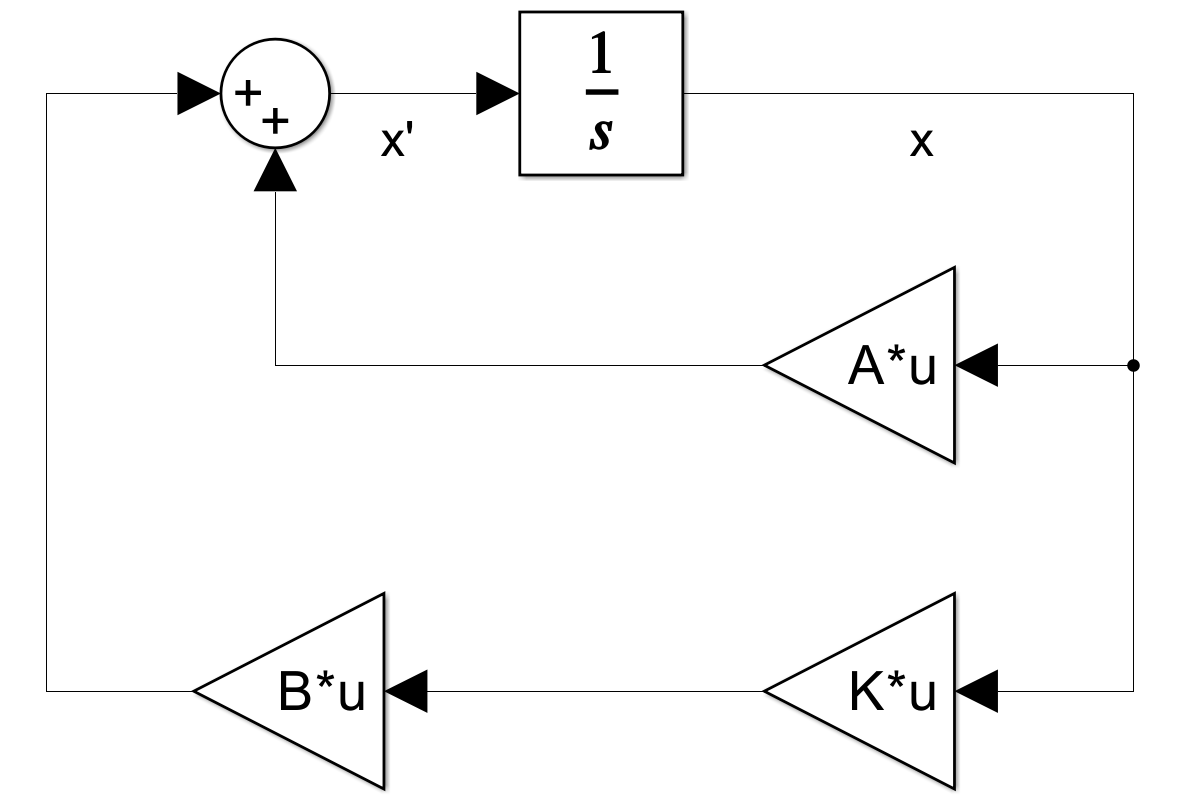
\includegraphics[width=0.8\textwidth]{figs/task1_slx.png}
    \caption{Схема моделирования системы \eqref{eq:sys1} с регулятором $u=-Kx$}
    \label{fig:sys1}
\end{figure}

Зададимся парой значений степени устойчивости $\alpha_1=2$ и $\alpha_2=0.2$
для дальнейшего их исследования.



\subsection{Степень устойчивости 1}

\subsubsection{Синтез регулятора при помощи матричного неравенства
типа Ляпунова}

Синтезируем регулятор со степенью устойчивости $\alpha_1=2$ при помощи
матричного неравенства типа Ляпунова
\begin{equation}
    PA^T+AP+2\alpha P+Y^TB^T+BY\preccurlyeq0,\quad P\succ0,\quad K=YP^{-1}.
    \label{eq:lyap}
\end{equation}
Найдем матрицу регулятора $K_1$, обеспечивающую желаемую степень 
устойчивости без ограничений на управление, для этого воспользуемся CVX, 
используя неравенства \eqref{eq:lyap}. Получаем
\begin{equation*}
    K_1=\begin{bmatrix}
        3.3536&	2.1216&	-17.9071
    \end{bmatrix}.
\end{equation*}
Найдем матрицу регулятора $K_2$, обеспечивающую желаемую степень 
устойчивости совместно с решением задачи минимизации управления,
для этого понадобятся еще пара неравенств:
\begin{equation}
    \begin{bmatrix}
        P&x_0\\
        x_0^T&1
    \end{bmatrix}\succ0,\quad
    \begin{bmatrix}
        P&Y^T\\
        Y&\gamma I
    \end{bmatrix}\succ0,
\end{equation}
минимизировать нужно $\gamma$, начальное состояние возьмем 
нулевым (оно большой роли не играет, насколько я понимаю), и, используя CVX, получим
\begin{equation*}
    K_2=\begin{bmatrix}
        -1.0712&	-1.0712&	-3.3288
    \end{bmatrix}.
\end{equation*}


\subsubsection{Синтез регулятора при помощи матричного
уравнения типа Риккати}

Уравнение Риккати выглядит следующим образом
\begin{equation}
    A^TP+PA+Q-vPBR^{-1}B^TP+2\alpha P=0,\quad K=-R^{-1}B^TP
\end{equation}
при этом для работы регулятора необходимо $P\succ0$. Нас интересует его форма когда
$v=2$ и $R=1,$ тогда уравнение выглядит следующим образом
\begin{equation}
    A^TP+PA+Q-2PBB^TP+2\alpha P=0,\quad K=-B^TP.
    \label{eq:ric}
\end{equation}
Находить решение будем через vpasolve, а для этого нужно ``урезать'' систему,
чтобы она стала полностью управляемой. Жорданова форма систему выглядит
следующим образом
\begin{equation*}
    A_J=\begin{bmatrix}
        -2&0&0\\
        0&2&-1\\
        0&1&2
    \end{bmatrix},\quad
    B_J=\begin{bmatrix}
        0\\0.7071\\-2.1213
    \end{bmatrix},\quad
    P=\begin{bmatrix}
        -1&	0.7071&	-0.7071\\
        1&	-1.4142&	0\\
        0&	1.4142&	0
    \end{bmatrix}.
\end{equation*}
``Урезанная'' версия:
\begin{equation*}
    A_j=\begin{bmatrix}
        2&-1\\
        1&2
    \end{bmatrix},\quad
    B_j=\begin{bmatrix}
        0.7071\\-2.1213
    \end{bmatrix}
\end{equation*}
Теперь с помощью vpasolve найдем матрицу регулятора, решив уравнение \ref{eq:ric}
и взяв за $Q$ единичную матрицу,
\begin{equation*}
    K_{3_j}=\begin{bmatrix}
        16.6595& -1.5221
    \end{bmatrix},
\end{equation*}
дополним ее
\begin{equation*}
    K_{3_J}=\begin{bmatrix}
        0&16.6595& -1.5221
    \end{bmatrix},
\end{equation*}
и найдем ее в исходном базисе
\begin{equation*}
    K_3=K_{3_J}P^{-1}=\begin{bmatrix}
        2.1526&2.1526& -10.7037
    \end{bmatrix}.
\end{equation*}
Теперь возьмем за $Q$ нулевую матрицу, было найдено решение
\begin{equation*}
    K_{4_j}=\begin{bmatrix}
        -14.7078& -1.1314
    \end{bmatrix},
\end{equation*}
найдем матрицу в исходном базисе
\begin{equation*}
    K_4=K_{4_J}P^{-1}=\begin{bmatrix}
        1.6&1.6& -9.6
    \end{bmatrix}.
\end{equation*}



\subsubsection{Проверка регуляторов}

Найдем собственные числа матриц замкнутых систем
\begin{equation*}
    \sigma(A+BK_1)=\{\ -4.6608 \pm 3.6560i,\ -2\ \},\quad
    \sigma(A+BK_2)=\{\ -2 \pm 2.8798i,\ -2\ \},
\end{equation*}
\begin{equation*}
    \sigma(A+BK_3)=\{\ -2.2755 \pm 4.3745i,\ -2\ \},\quad
    \sigma(A+BK_4)=\{\ -2 \pm 4.1231i,\ -2\ \}.
\end{equation*}
Как видно, система стала устойчивой с желаемой степенью. При нахождении
регулятора без ограничения управления собственные числа получились какие-то ``случайные''
и даже более ``устойчивые'' чем требуется; при минимизации управления, собственные
числа подобрались минимально возможные для удовлетворения желаемой степени устойчивости.




\subsubsection{Моделирование}

Для обеих замкнутых систем выполнить компьютерное моделирование,
построим графики формируемых регуляторами управлений $u(t)$ и векторов
состояния замкнутых систем $x(t)$ при начальных условиях $x(0) =\begin{bmatrix}
    1&1&1
\end{bmatrix}^T$ (см \autoref{fig:1k1}). Как видно по графикам, управление
при регуляторе $K_2$, который синтезировался с ограничением управления, менее
``сильное'' в сравнении с регулятором $K_1$, что заметно отражается на 
скорости сходимости состояния к точке равновесия.

\begin{figure}[H]
    \centering
    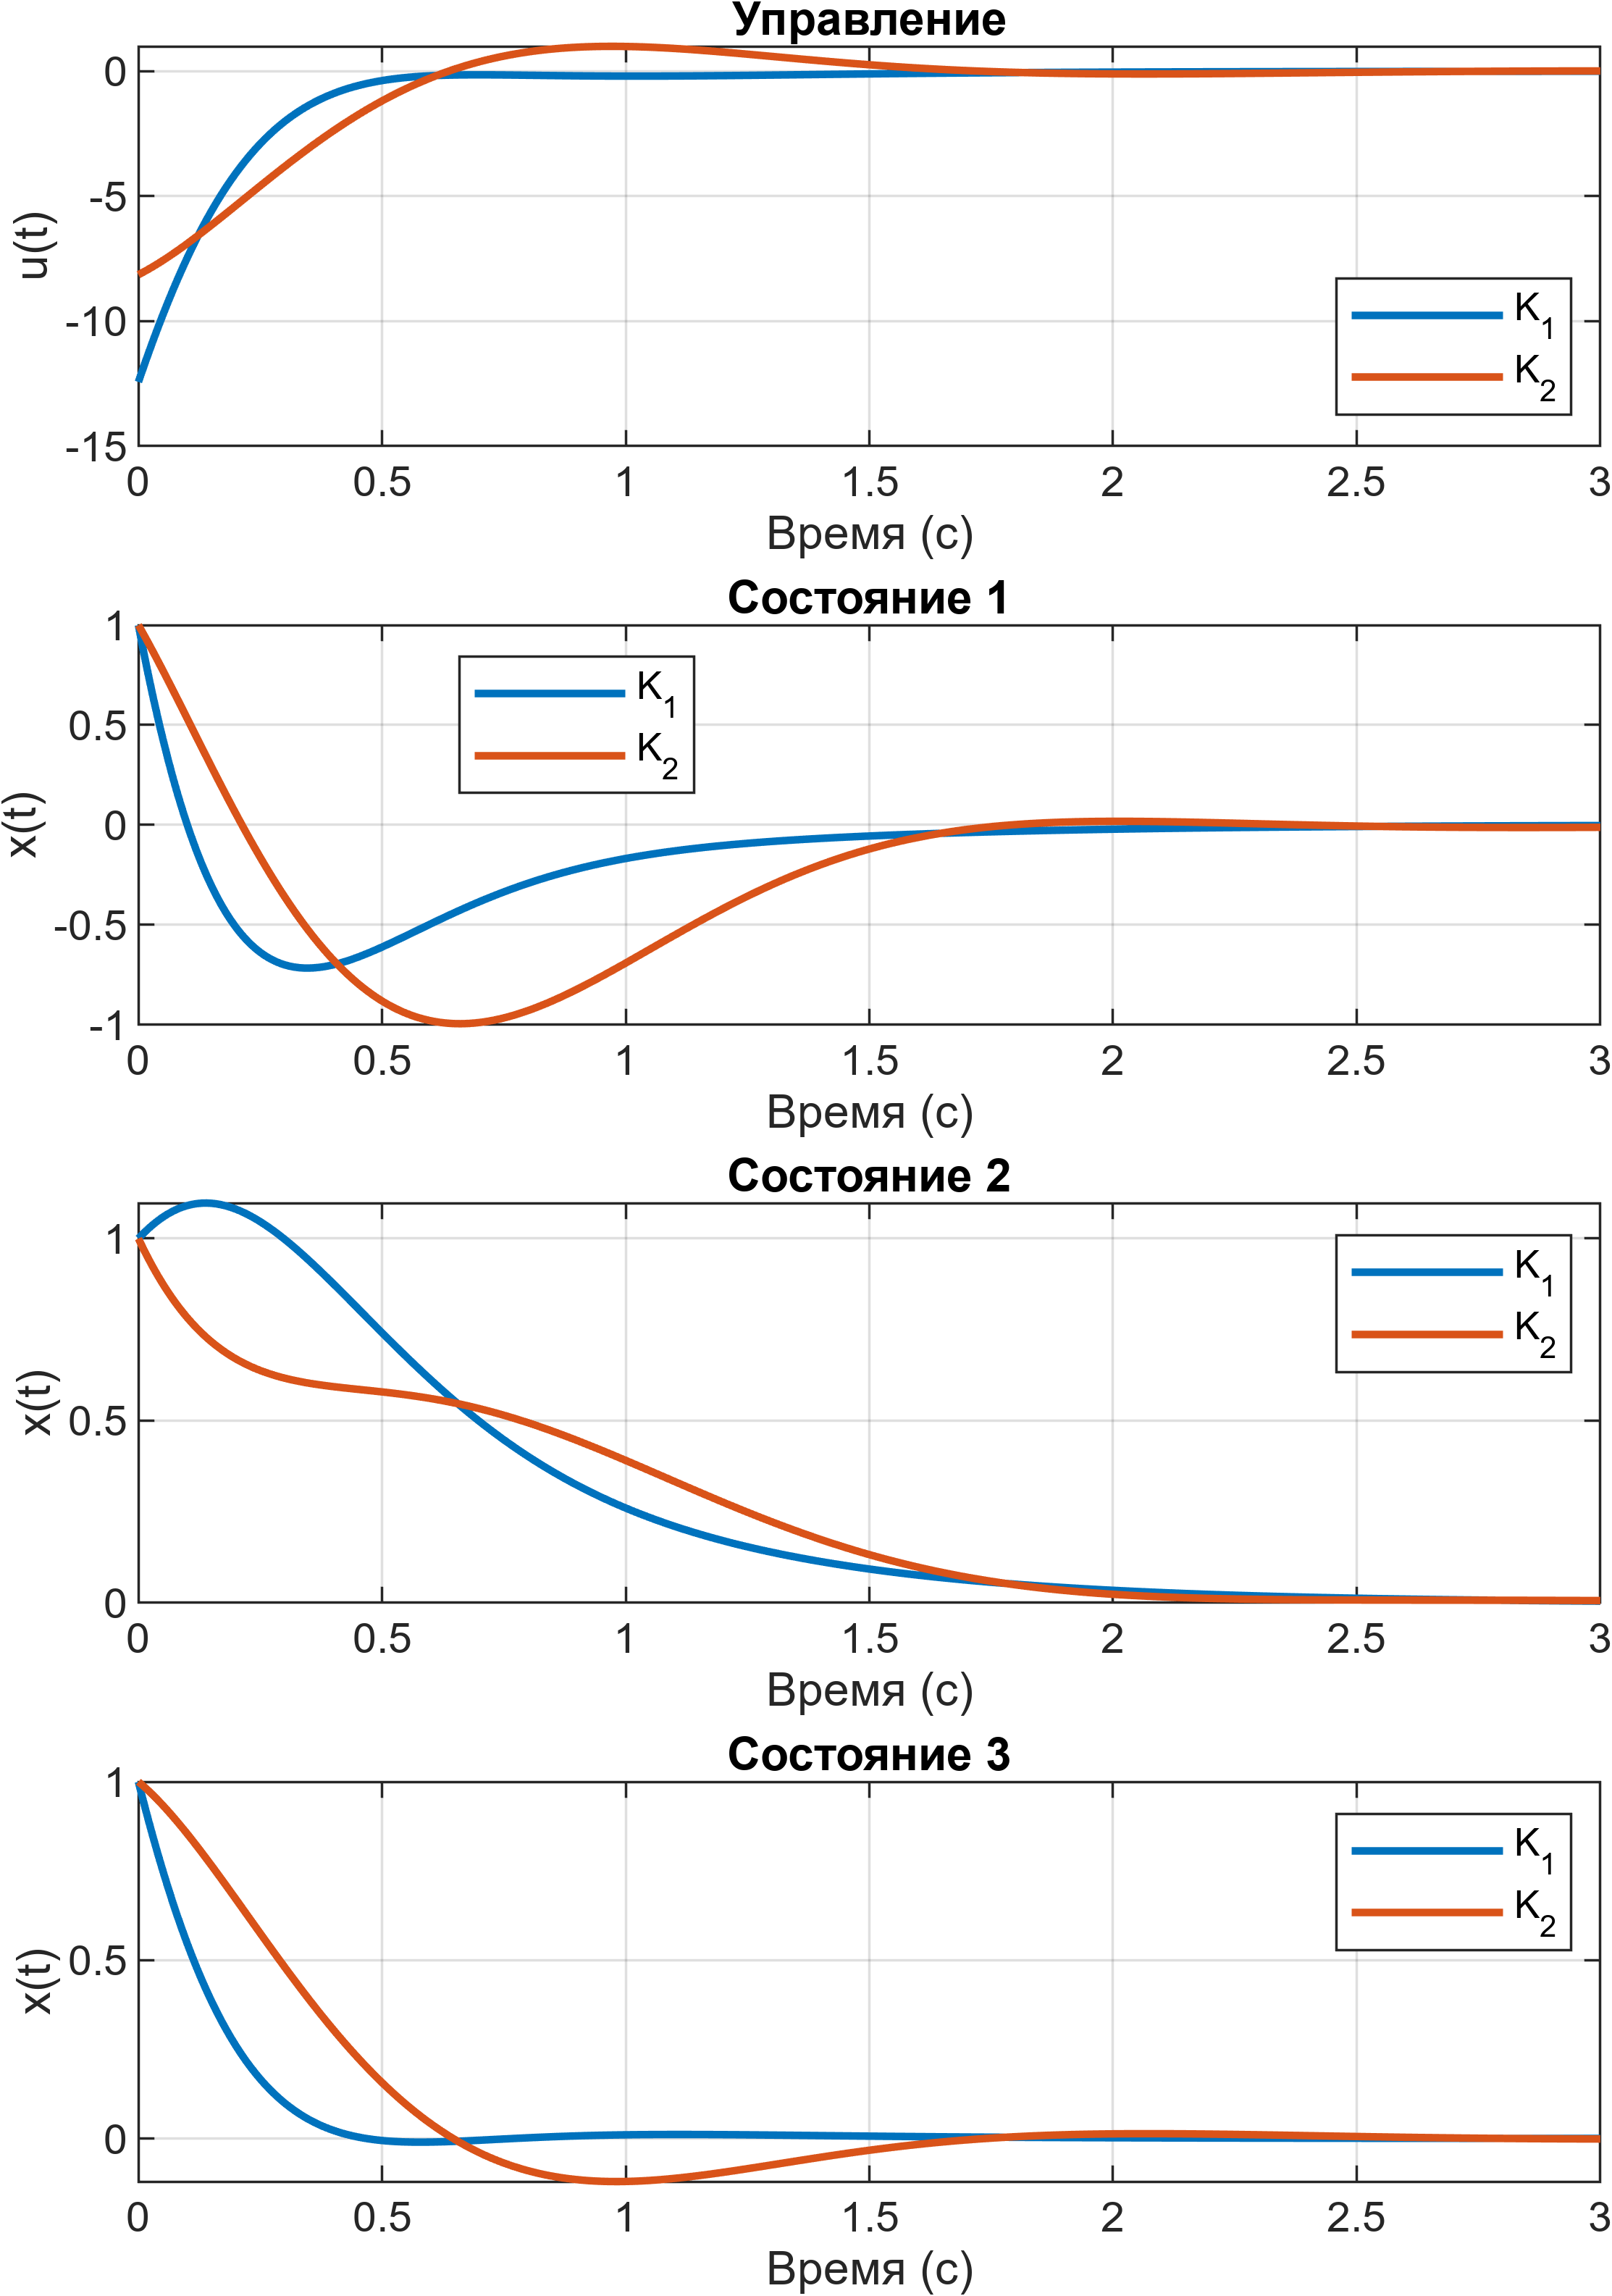
\includegraphics[width=\linewidth]{figs/task10.png}
    \caption{Моделирование системы \eqref{eq:sys1} с регулятором вида $u=Kx$
    со степенью устойчивости $\alpha=2$}
    \label{fig:1k1}
\end{figure}




\subsection{Степень устойчивости 2}

\subsubsection{Синтез регулятора}

Аналогично синтезируем регулятор со степенью устойчивости $\alpha_1=0.2$.
Найдем матрицу регулятора $K_1$, обеспечивающую желаемую степень 
устойчивости без ограничений на управление, для этого воспользуемся CVX и получим
\begin{equation*}
    K_1=\begin{bmatrix}
        -1.6329&	-2.3204&	-9.5054
    \end{bmatrix}.
\end{equation*}
Найдем матрицу регулятора $K_2$, обеспечивающую желаемую степень 
устойчивости совместно с решением задачи минимизации управления,
начальное состояние так же возьмем нулевым, и, используя CVX, получим
\begin{equation*}
    K_2=\begin{bmatrix}
        -1.0712&	-1.0712&	-3.3288
    \end{bmatrix}.
\end{equation*}


\subsubsection{Проверка регулятора}

Найдем собственные числа матриц замкнутых систем
\begin{equation*}
    \sigma(A+BK_1)=\{\ -1.4599,\    -4.9909,\    -2.0000\ \},\quad
    \sigma(A+BK_2)=\{\ -0.2000 \pm 2.0010i,\ -2\ \}.
\end{equation*}
Как видно, система стала устойчивой с желаемой степенью. 
Как и с предыдущей степенью устойчивости, при нахождении
регулятора без ограничения управления собственные числа получились ``случайные''
и более ``устойчивые'' чем требуется; при минимизации управления, собственные
числа подобрались минимально возможные для удовлетворения желаемой степени устойчивости.


\subsubsection{Моделирование}

Для обеих замкнутых систем выполнить компьютерное моделирование,
построим графики формируемых регуляторами управлений $u(t)$ и векторов
состояния замкнутых систем $x(t)$ при начальных условиях $x(0) =\begin{bmatrix}
    1&1&1
\end{bmatrix}^T$ (см \autoref{fig:2k1}). Как видно по графикам, управление
при регуляторе $K_2$ гораздо менее ``сильное'' в сравнении с регулятором $K_1$, 
что крайне заметно отражается на скорости сходимости состояния к точке равновесия,
объясняется это желаемой степенью устойчивости, которая в 10 раз меньше предыдущей,
и когда она точно соблюдается (при минимизации управления) мы получаем систему,
сходящуюся примерно во столько же раз медленнее.

\begin{figure}[H]
    \centering
    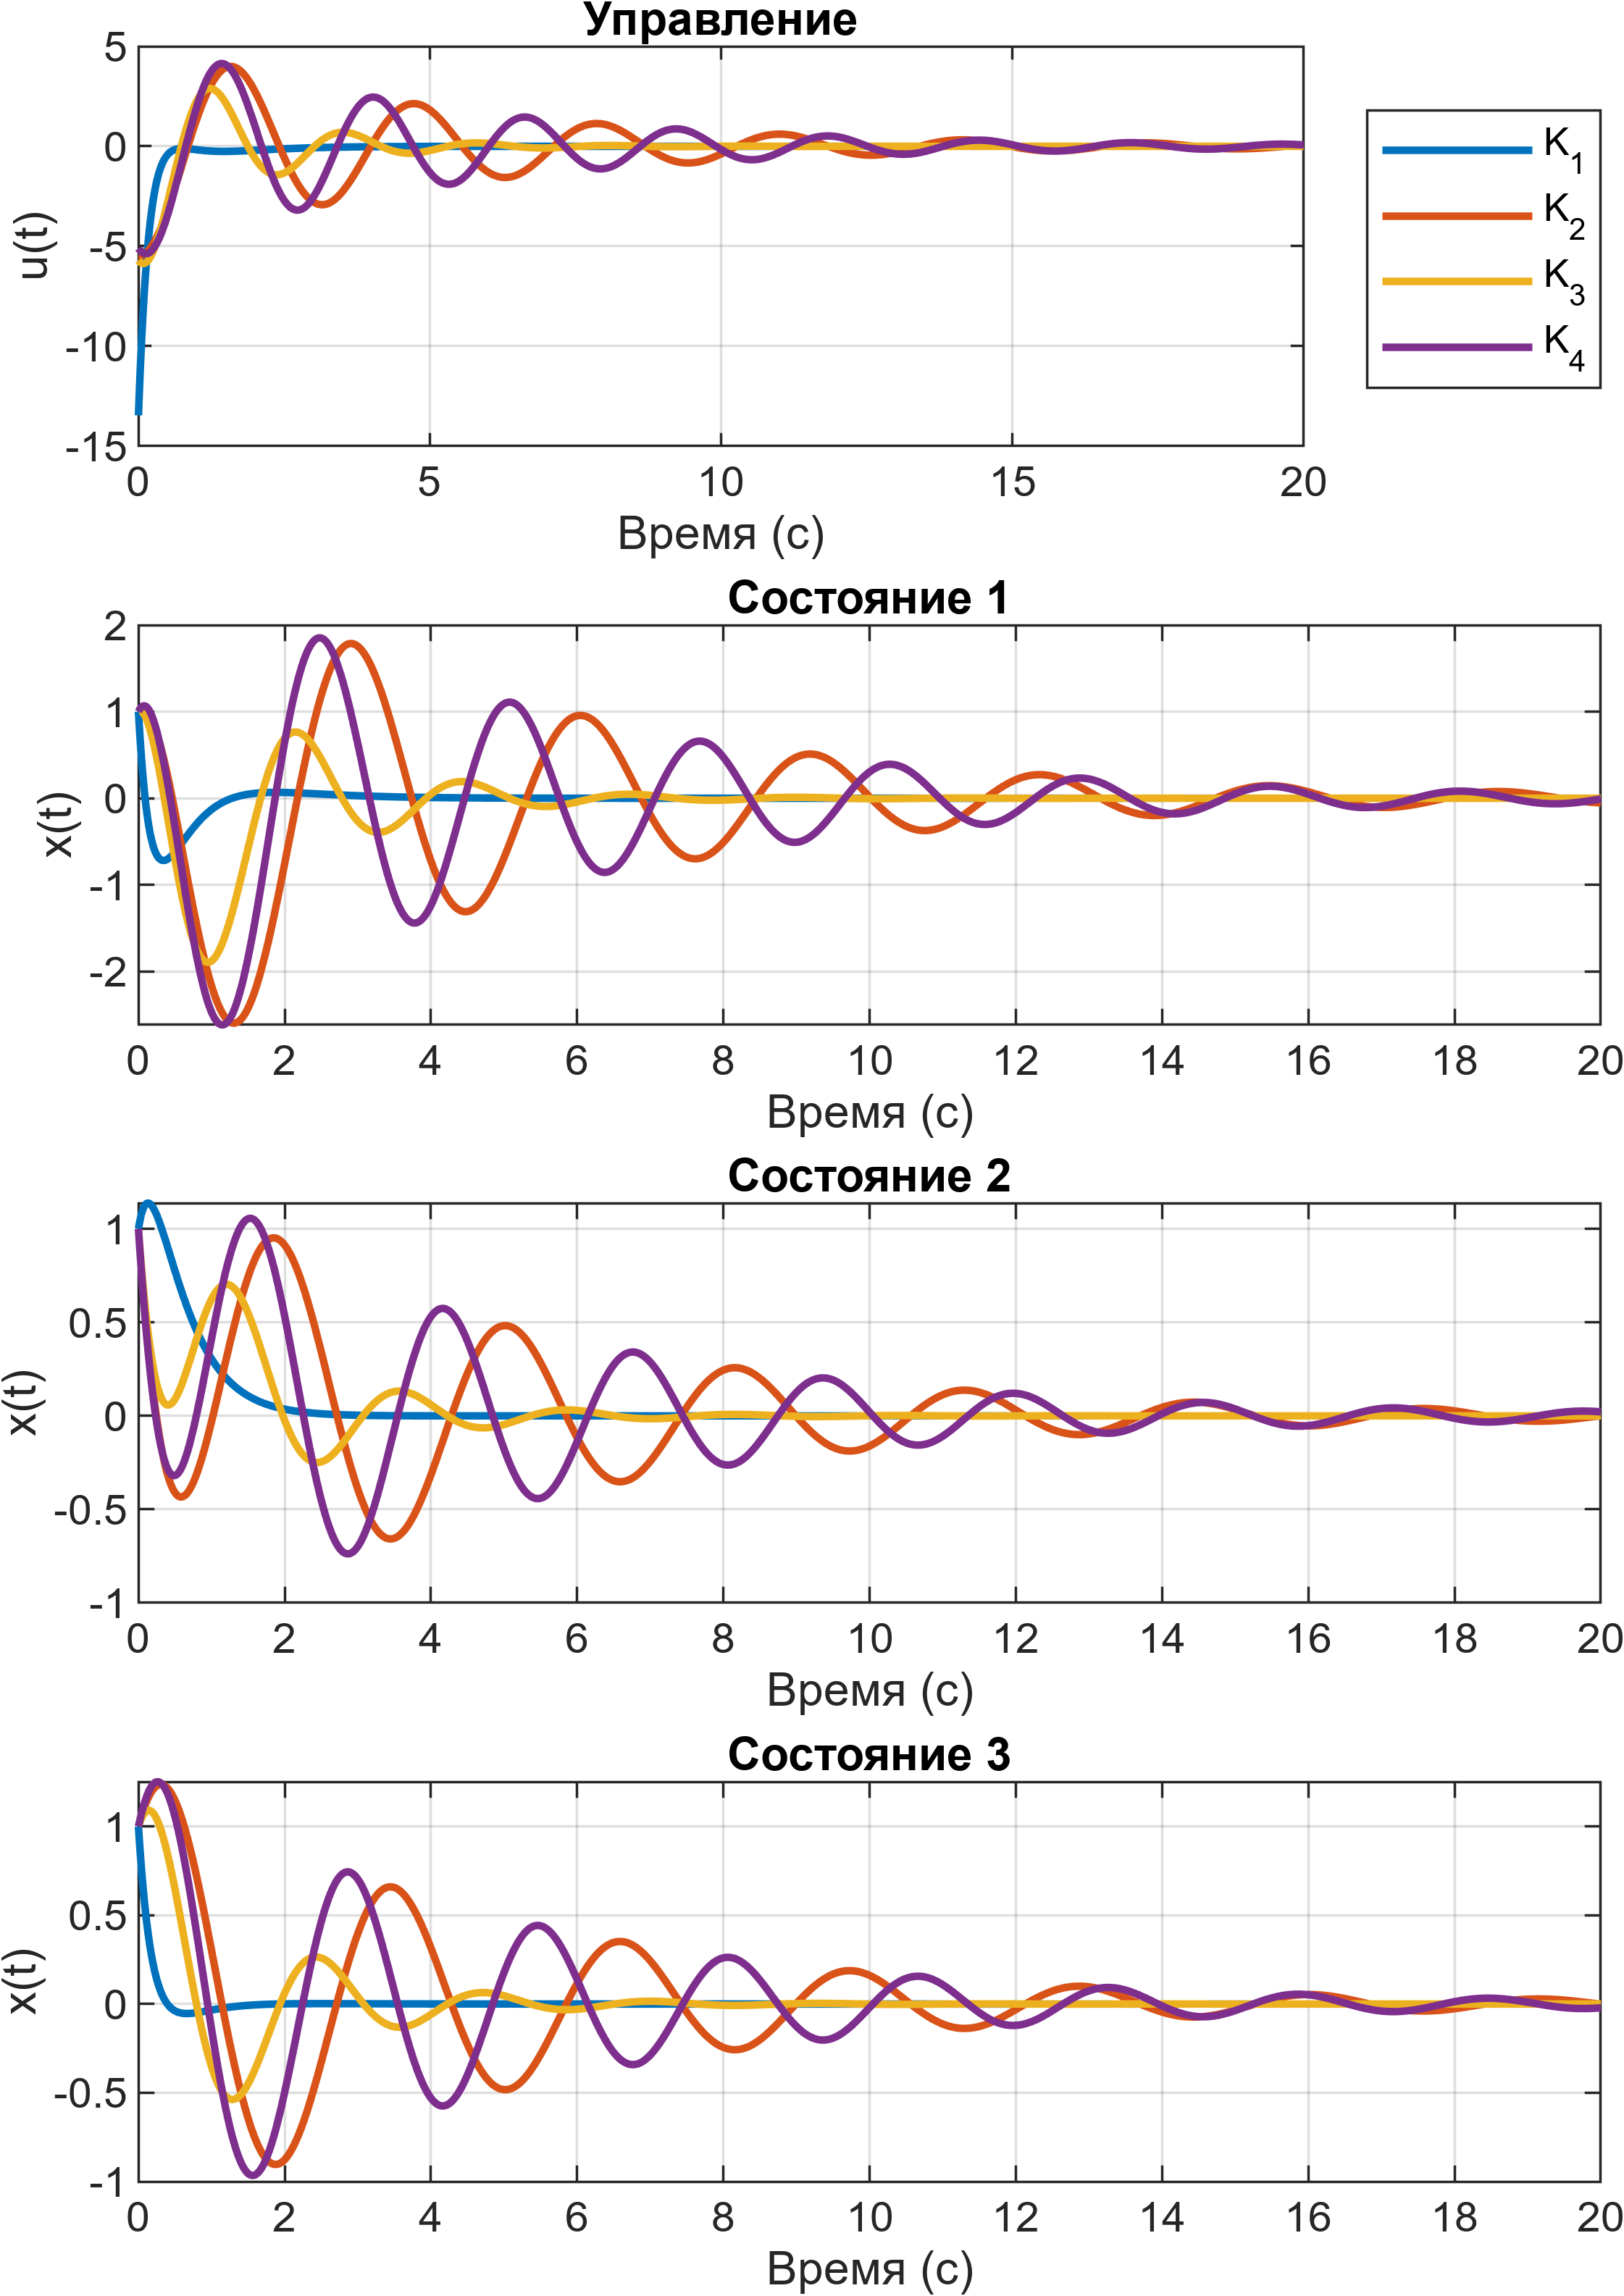
\includegraphics[width=\linewidth]{figs/task11.png}
    \caption{Моделирование системы \eqref{eq:sys1} с регулятором вида $u=Kx$
    со степенью устойчивости $\alpha=0.2$}
    \label{fig:2k1}
\end{figure}



